\newpage

\appendix \addcontentsline{toc}{section}{Appendix}

    \section{Appendix A: Schematics} \label{appendix:schematics}

        \begin{figure}[ht]
            \begin{center}
                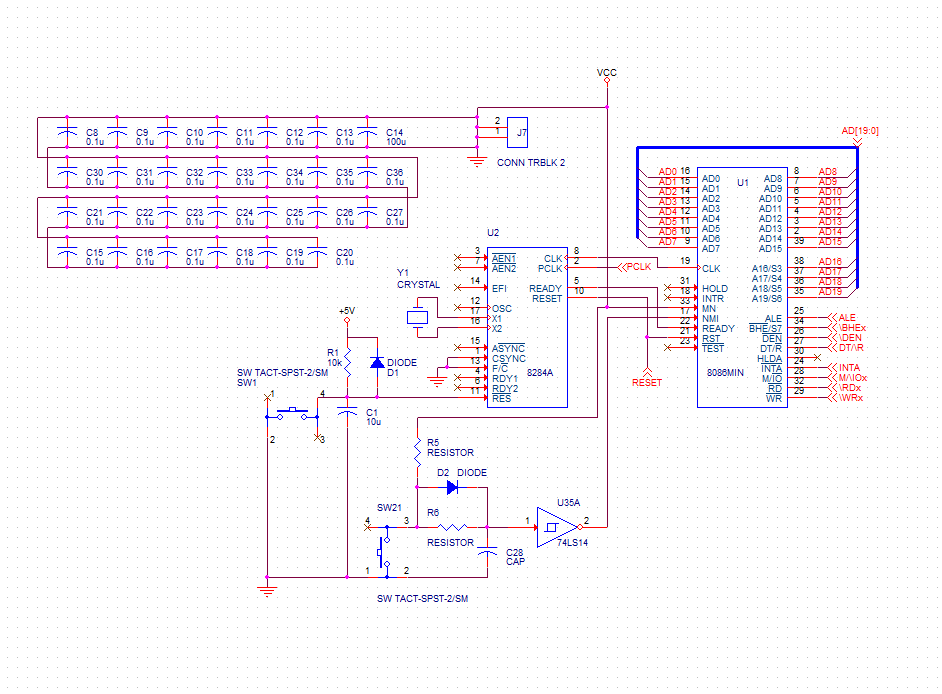
\includegraphics[width=1\textwidth]{figures/schematics/page1.png}
                \caption{8086 interfaced with the 8284A clock generator and its Reset RC Push Button Circuit, and the Power Bank of the Board} \label{fig:page1}
            \end{center}
        \end{figure}

        \begin{figure}[ht]
            \begin{center}
                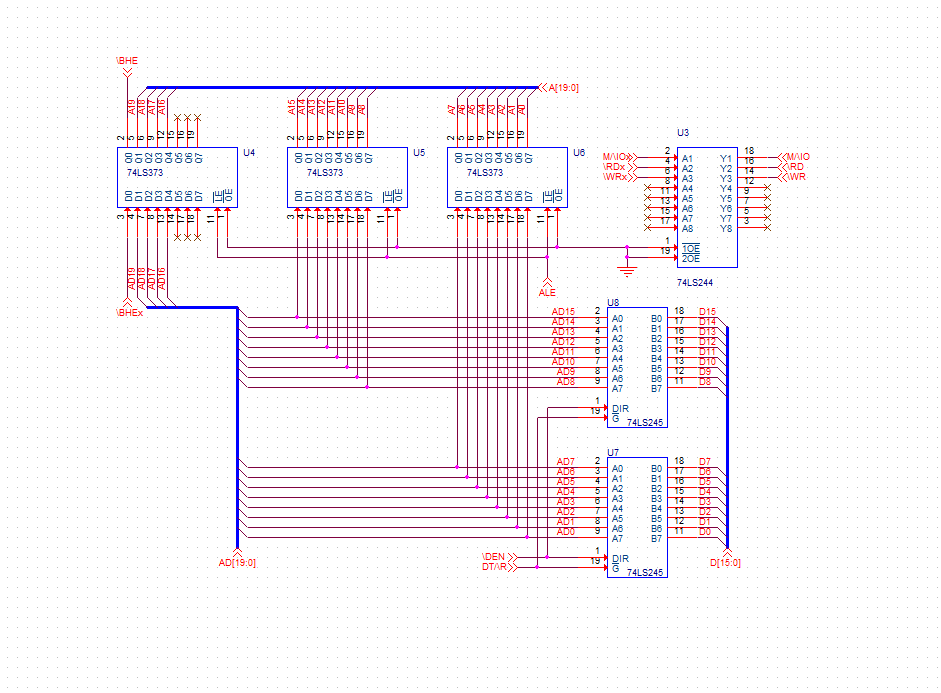
\includegraphics[width=1\textwidth]{figures/schematics/page2.png}
                \caption{8086 Demultiplexed with Address and Data Buses Pulled into Headers} \label{fig:page2}
            \end{center}
        \end{figure}

        \begin{figure}[ht]
            \begin{center}
                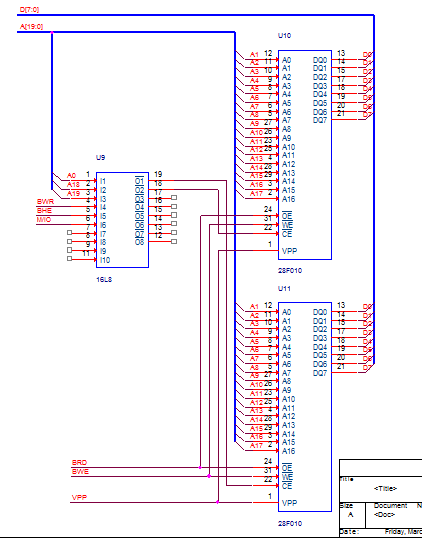
\includegraphics[width=1\textwidth]{figures/schematics/page3.png}
                \caption{256 kB of CMOS Flash Memory and 128 kB Static SRAM} \label{fig:page3}
            \end{center}
        \end{figure}

        \begin{figure}[ht]
            \begin{center}
                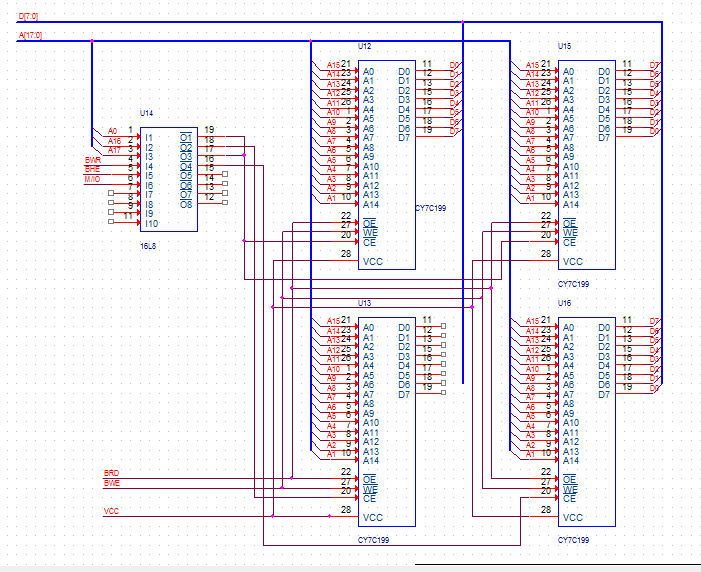
\includegraphics[width=1\textwidth]{figures/schematics/page4.png}
                \caption{128 kB Static SRAM} \label{fig:page4}
            \end{center}
        \end{figure}

        \begin{figure}[ht]
            \begin{center}
                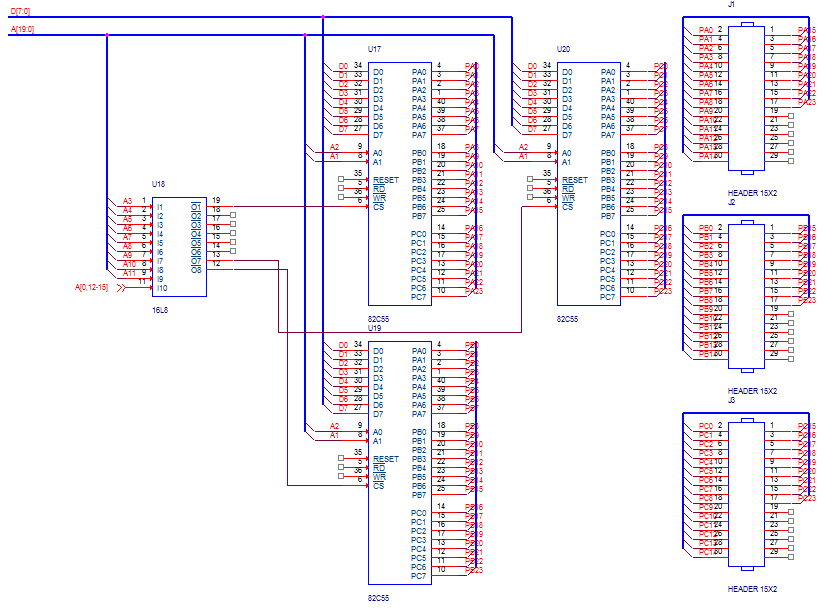
\includegraphics[width=1\textwidth]{figures/schematics/page5.png}
                \caption{Programmable Peripheral Interface Chips with Port Connections Pulled into Headers} \label{fig:page5}
            \end{center}
        \end{figure}

        \begin{figure}[ht]
            \begin{center}
                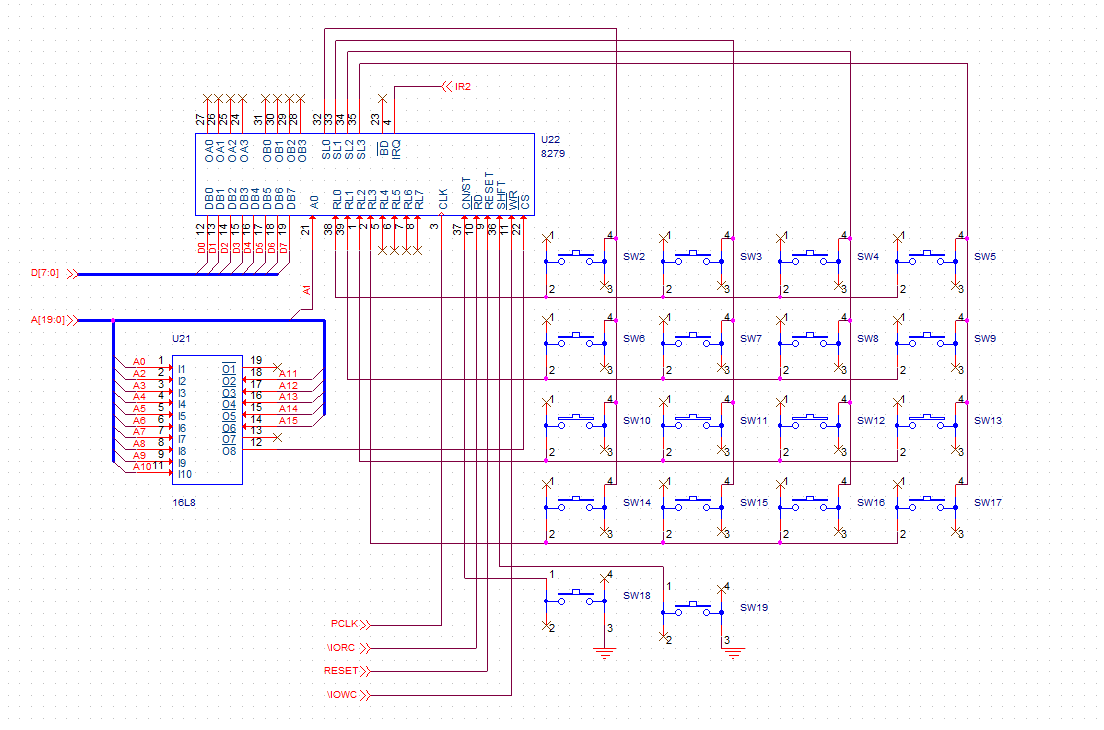
\includegraphics[width=1\textwidth]{figures/schematics/page6.png}
                \caption{5$\times$4 Keyboard Matrix} \label{fig:page6}
            \end{center}
        \end{figure}

        \begin{figure}[ht]
            \begin{center}
                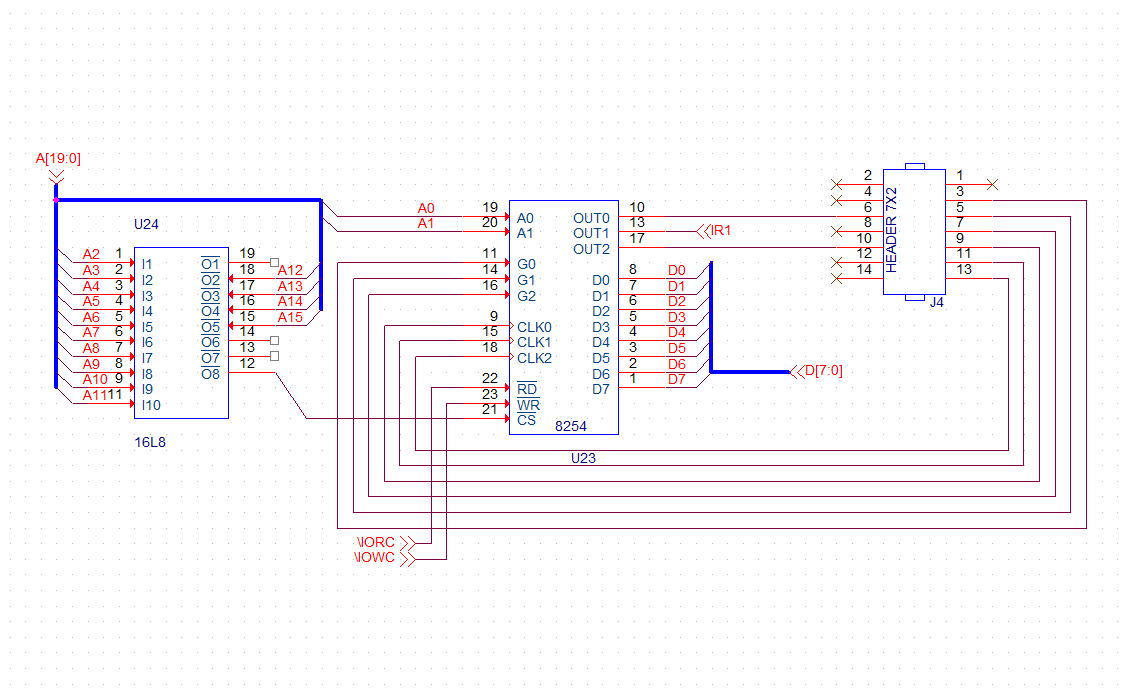
\includegraphics[width=1\textwidth]{figures/schematics/page7.png}
                \caption{Programmable Interval Timer} \label{fig:page7}
            \end{center}
        \end{figure}

        \begin{figure}[ht]
            \begin{center}
                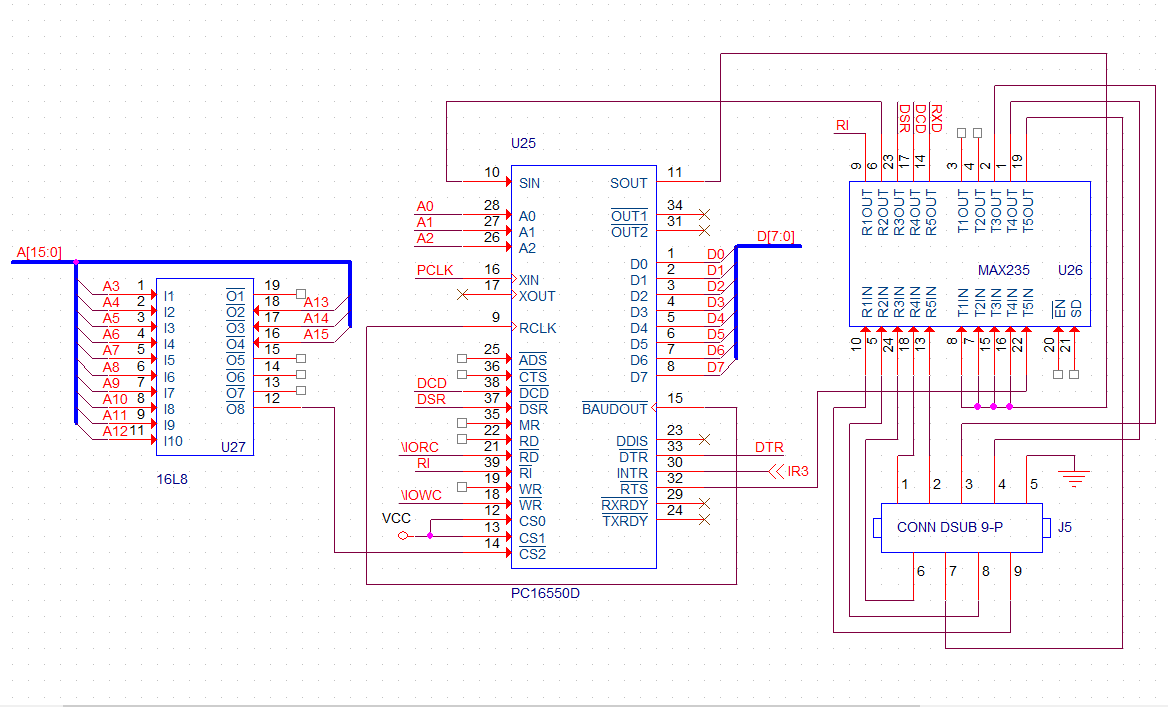
\includegraphics[width=1\textwidth]{figures/schematics/page8.png}
                \caption{UART Connected for Serial Port Using a Line Driver/Receiver and a DSUB-9 connector} \label{fig:page8}
            \end{center}
        \end{figure}

        \begin{figure}[ht]
            \begin{center}
                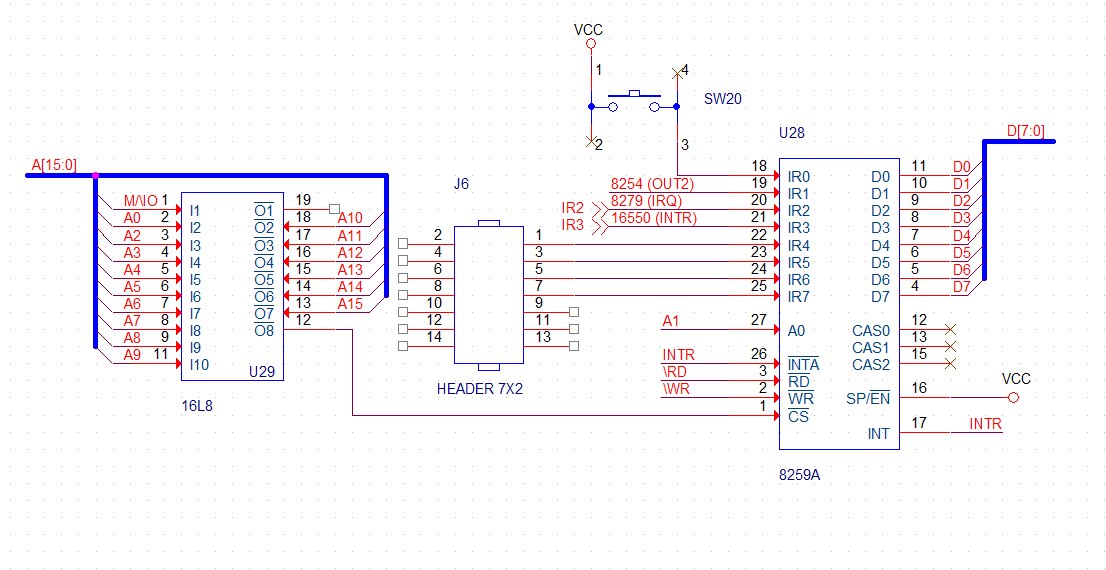
\includegraphics[width=1\textwidth]{figures/schematics/page9.png}
                \caption{Programmable Interrupt Controller with Headers fro External Access} \label{fig:page9}
            \end{center}
        \end{figure}

        \begin{figure}[ht]
            \begin{center}
                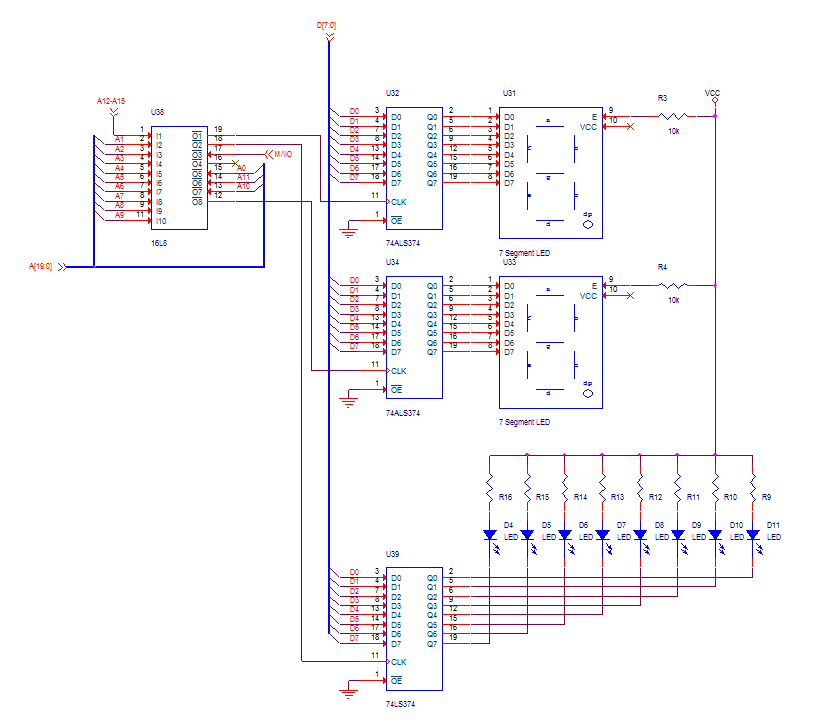
\includegraphics[width=1\textwidth]{figures/schematics/page10.png}
                \caption{Common-Anode 7-Segment LEDs with 8 LEDs} \label{fig:page10}
            \end{center}
        \end{figure}

        \begin{figure}[ht]
            \begin{center}
                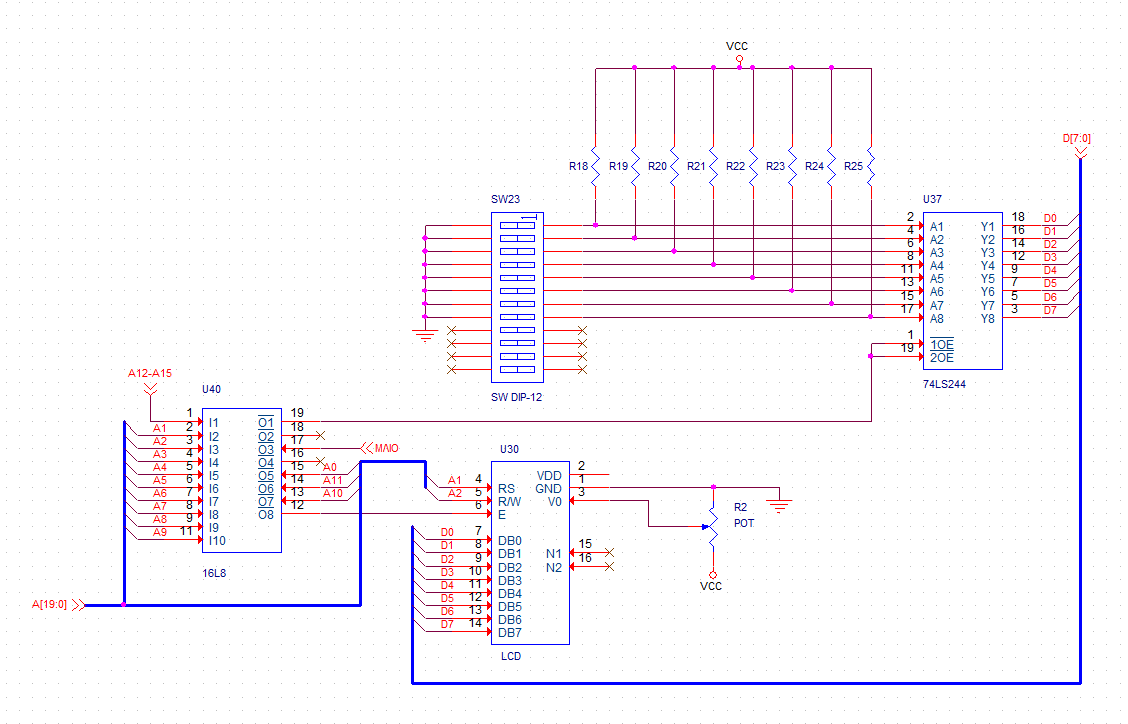
\includegraphics[width=1\textwidth]{figures/schematics/page11.png}
                \caption{20 character $\times$ 4 line LCD Display with an Integrated LCD Controller} \label{fig:page11}
            \end{center}
        \end{figure}


    \clearpage
    \newpage

    \section{Appendix B: Pinouts} \label{appendix:pinouts}

        \subsection{8086 Chip}

                \begin{itemize}

                    \item $M/\overline{IO}$: (Memory/ I/O) indicates if the address is a memory or I/O address

                    \item $\overline{INTA}$: (Interrupt Acknowledgment) generated in response to $INTR$ to put the interrupt vector on the data bus

                    \item $ALE$: (Address Latch Enable) when 1, address data bus contains a memory or I/O address

                    \item $\overline{DEN}$: (Data Bus Enable) activates external data bus buffers

                \end{itemize}


    \clearpage
    \newpage

    \section{Appendix C: Code Implementations} \label{appendix:code}

        \subsection{Programmable Logic Devices}

            \subsubsection{U9}

                \VerbatimInput{hdl/u09.vhd}

            \newpage
            \subsubsection{U14}

                \VerbatimInput{hdl/u14.vhd}

            \newpage
            \subsubsection{U18}

                \VerbatimInput{hdl/u18.vhd}

            \newpage
            \subsubsection{U21}

                \VerbatimInput{hdl/u21.vhd}

            \newpage
            \subsubsection{U24}

                \VerbatimInput{hdl/u24.vhd}

            \newpage
            \subsubsection{U27}

                \VerbatimInput{hdl/u27.vhd}

            \newpage
            \subsubsection{U29}

                \VerbatimInput{hdl/u29.vhd}

            \newpage
            \subsubsection{U38}

                \VerbatimInput{hdl/u38.vhd}

            \newpage
            \subsubsection{U40}

                \VerbatimInput{hdl/u40.vhd}

        \newpage
        \subsection{Assembly Implementations}

            \subsubsection{LCD} \label{sec:lcd_asm}
                \VerbatimInput{assembly/lcd.asm}

